\item

\begin{multicols}{2}

Der Grad des nebenstehenden Polynoms $p(x)$ beträgt wenigstens $4$. Warum? Finden Sie unter der Annahme, der Grad betrage genau $4$, eine mögliche Funktionsgleichung für $p(x)$! (Hinweis: Lesen Sie einige gut erkennbare Punkte von $f$ ab.) 

\columnbreak

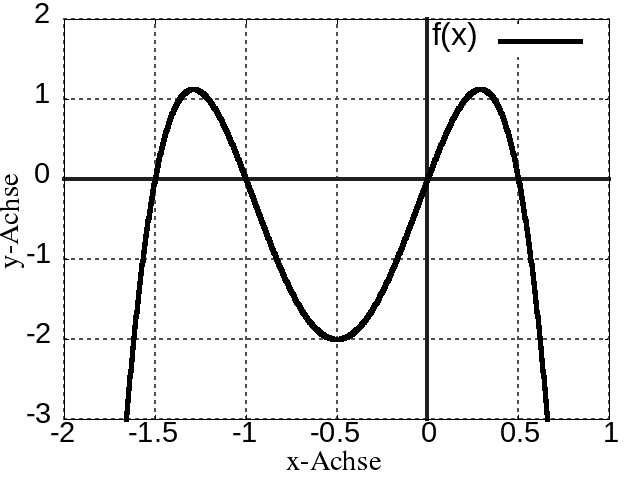
\includegraphics[width=0.35\textwidth]{../pool/ex-graph-read-2-img-a.png}

\end{multicols}

